paragraph{More Examples : }

Now consider the simple code excerpt below.

\begin{verbatim}

00	r3 <- r5 op r6
10	r1 <- r3 op r1
20	r3 <- r5 op r6

\end{verbatim}

In this example we assume that instruction 10 and 20 get to execute
before instruction 00 does.  We will also assume that instructions
00 and 10 both execute in the same clock cycle.
Initially, as always, the sources for these instructions
are taken from the ISA register file at load time.

Firstly, it should be noted that after instruction 10
executes at least once, it will not necessarily be enabled to execute
again even though one of its input sources has changed ; namely,
register
{\tt r1}.
It is not enabled to execute again for this input source change because
the new value of
{\tt r1}
that is generated is only forwarded to instructions {\it later}
in time order than instruction 10.  
Instruction 10 will never, therefor, see register
{\tt r1}
being updated due to its own broadcast of that register.

In like manner, instruction
10 will not be enabled to execute simply because of the register change
of
{\it r3}
from instruction 20.  The output from instruction 20 will
only be broadcast forward to later active stations and
the active station holding instruction 10 is not snooping for it.

Finally, when instruction 00 does get to execute, it will
forward broadcast an updated value for register
{\it r3}.
Since instruction 10 is snooping on changes to this value,
it will be enabled to execute again and will eventually do so.
The execution of instruction 10 relative to instructions
00 and 20 might appear as shown in
Figure~\ref{ex3}.

\begin{figure}
\centering
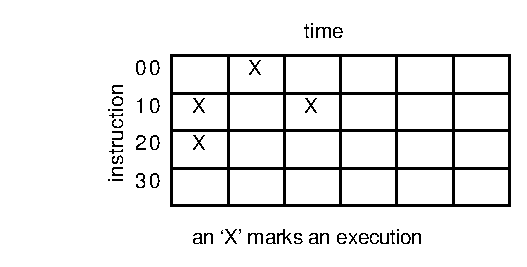
\epsfig{file=e3.eps,width=2.50in}
\caption{{\em Timing of the code example, scenario 3.}
In this example instruction 10 does not re-execute due to an update
of its input register from instructions 10 and 20 but does
finally re-execute after an update from instruction 00.
Execution of an instruction at a given time is
again indicated by an `X'.}
\label{ex3}
\end{figure}




